% main.tex — Rapport « Le jeu du seau d'eau » (≤ 5 pages) : implémentation et
% physique du mode jeu de l'exercice du looping avec wagon
% (src/mechanics/loop-wagon/game.js). Les chiffres viennent du code via
% outils/donnees.mjs, les captures via outils/captures.cjs.
% Compilation : powershell -ExecutionPolicy Bypass -File memoire\rapport-jeu-seau\compiler.ps1

\documentclass[10pt, a4paper]{article}

\usepackage[T1]{fontenc}
\usepackage[utf8]{inputenc}
\usepackage{lmodern}
\usepackage[english, french]{babel}
\usepackage{microtype}
\usepackage[a4paper, margin=2cm]{geometry}
\usepackage{amsmath, amssymb}
\usepackage[locale=FR]{siunitx}
\usepackage{graphicx}
\usepackage{subcaption}
\usepackage{placeins}
\usepackage{booktabs}
\usepackage{xcolor}
\usepackage{tikz}
\usetikzlibrary{arrows.meta, calc, babel}
\usepackage{pgfplots}
\pgfplotsset{compat=1.18}
\usepackage{csquotes}
\usepackage[backend=biber, style=ieee, autolang=other]{biblatex}
\usepackage[hidelinks]{hyperref}
\usepackage[nameinlink]{cleveref}
\addbibresource{references.bib}
\crefname{table}{tableau}{tableaux}
\Crefname{table}{Tableau}{Tableaux}
\graphicspath{{figures/}}

\definecolor{accent}{HTML}{1976D2}
\definecolor{poids}{HTML}{D32F2F}
\definecolor{tensionc}{HTML}{8E24AA}
\definecolor{corde}{HTML}{8D6E63}
\definecolor{eau}{HTML}{1E88E5}
\definecolor{metal}{HTML}{546E7A}

\newcommand{\vect}[1]{\boldsymbol{#1}}
\setlength{\parskip}{0.35em}
\setlength{\parindent}{0pt}

\title{\vspace{-1.5cm}Le jeu du seau d'eau : implémentation et physique}
\author{Arnaud \textsc{Gheysens}\thanks{Rédigé avec l'aide d'une IA ; voir la page « Utilisation de l'intelligence artificielle dans le projet ».}}
\date{Mémoire — rapport technique, novembre 2026}

\begin{document}
\maketitle
\vspace{-0.6cm}

% 01-defi.tex — Le défi et la théorie du cours (vitesse minimale, tension maximale).

\section{Le défi et la théorie du cours}

Le mode jeu de l'exercice du looping propose une expérience que chacun connaît :
faire tourner un seau d'eau dans un plan vertical sans se mouiller. Une barre
tourne autour d'un pivot ; une corde pend à son bout et porte un seau rempli
d'eau. L'étudiant règle une seule grandeur, tirée au sort à chaque défi : la
vitesse \(v_0\) du seau au point bas, la longueur \(L\) de la corde ou la masse
\(m\) du seau rempli. Le défi est réussi si le seau fait deux tours sans perdre
une goutte ni casser la corde (\cref{fig-captures}).

Dans le cours, le seau est un point matériel au bout d'une corde sans masse,
à la distance \(R\) du pivot. La conservation de l'énergie donne la vitesse à
l'angle \(\theta\) compté depuis le point bas,
\(v^2 = v_0^2 - 2 g R (1 - \cos(\theta))\), et la deuxième loi de Newton selon le
rayon donne la tension \cite{formulaire_epl1201} :
\begin{equation}
  T = m \left(\frac{v^2}{R} + g \cos(\theta)\right)
    = m \left(\frac{v_0^2}{R} + g \left(3 \cos(\theta) - 2\right)\right).
  \label{eq-tension}
\end{equation}
L'eau reste au fond tant que la corde tire (\(T > 0\)), et c'est au sommet
(\(\theta = \pi\)) que c'est le plus difficile :
\begin{equation}
  T_s = m \left(\frac{v_0^2}{R} - 5 g\right) \geq 0
  \quad \Longleftrightarrow \quad v_0 \geq \sqrt{5 g R} .
  \label{eq-sommet}
\end{equation}
C'est la condition du wagon dans le looping, \(h \geq 5R/2\), avec
\(v_0^2 = 2 g h\). La corde casse si la tension dépasse sa tension de rupture
\(T_{\max}\) ; la plus grande tension est au point bas,
\(m (v_0^2/R + g)\). L'étudiant calcule ces deux bornes. Ce rapport explique
comment le jeu simule le seau, la corde et l'eau, puis compare ce que la
simulation obtient à ce que ces formules prévoient.

% 02-modele.tex — Les objets simulés (barre, corde, seau, eau) et les choix qui
% demandent une explication.

\section{Les objets simulés}

La scène contient quatre objets (\cref{fig-schema}) ; hormis son poids, toutes
les forces sur le seau passent par la corde.
\begin{itemize}
  \item \emph{La barre} (\SI{0,9}{m}, \SI{0,3}{kg}) tourne sur un pivot sans
        frottement. Pour la rotation, une barre homogène de moment d'inertie
        \(m_b L_b^2/3\) équivaut à un point de masse \(m_b/3\) à son bout ; pour
        que le moment de son poids, \(m_b g (L_b/2) \sin(\alpha)\), soit juste,
        ce point subit une force \(m_b g/2\). Tant que le moteur la mène, sa
        position est imposée.
  \item \emph{La corde} (\SI{0,15}{kg/m}) est une chaîne de dix maillons qui
        peuvent raccourcir mais pas s'allonger : elle plie, se détend, ne pousse
        jamais. Son dernier nœud est l'anse du seau.
  \item \emph{Le seau} est un cylindre rigide (Ø \SI{26}{cm}, \SI{24}{cm} de
        profondeur, \SI{0,45}{kg}) avec son moment d'inertie (paroi et fond),
        pendu à une anse de \SI{0,05}{kg} qui pivote aux oreilles ; un petit
        frottement amortit ce pivot et le bout de la barre (\SI{8}{s^{-1}}).
  \item \emph{L'eau}, \(m - \SI{0,5}{kg}\) à \SI{1}{kg} par litre, est faite de
        dix billes par défaut, qui portent chacune un dixième de cette masse,
        roulent sur les parois, se poussent et poussent le seau. L'essai est
        raté dès qu'une bille franchit le bord.
\end{itemize}
Comme l'eau a une masse et une place, le centre de masse du seau rempli dépend
de la quantité d'eau. \(R\) est donc la distance du pivot au centre de masse
calculé sur les billes au repos : pour \(L = \SI{0,4}{m}\), \(R\) vaut \SI{1,585}{m} à \SI{0,6}{kg},
\SI{1,650}{m} à \SI{2}{kg} et \SI{1,622}{m} à \SI{8}{kg}
(\cref{tab-repos}). C'est ce \(R\) qui sert dans \(\sqrt{5 g R}\).

\begin{figure}[ht]
  \centering
  \begin{tikzpicture}[scale=1.05, every node/.style={font=\footnotesize}]
    \coordinate (pivot) at (0,0);
    \coordinate (tip) at (2.4,-1.2);
    \coordinate (anse) at (4.6,-2.45);
    \draw[metal!40, line width=3pt] (-0.5,-3.1) -- (pivot) -- (0.5,-3.1);
    \draw[metal, line width=2.6pt] (pivot) -- (tip);
    \fill (pivot) circle (2.4pt);
    \node[above left] at (pivot) {pivot};
    \node[above=2pt, sloped, metal] at ($(pivot)!0.35!(tip)$) {barre \(L_b\), \(m_b\)};
    \foreach \k in {1,...,9} { \coordinate (r\k) at ($(tip)!\k/10!(anse)+(0,-0.028*\k+0.0028*\k*\k)$); }
    \draw[corde, line width=1.1pt] (tip) \foreach \k in {1,...,9} { -- (r\k) } -- (anse);
    \foreach \k in {1,...,9} { \fill[corde] (r\k) circle (1.3pt); }
    \fill (tip) circle (1.8pt);
    \node[corde, above right] at ($(r4)+(0,0.08)$) {10 maillons \(\ell = L/10\), masse \(\mu \ell\) par nœud};
    \begin{scope}[shift={(anse)}, rotate=-30]
      \coordinate (ears) at (0,-0.42);
      \draw[black] (-0.34,-0.42) .. controls (-0.3,0.05) and (0.3,0.05) .. (0.34,-0.42);
      \draw[metal, very thick, fill=metal!10] (-0.34,-0.42) -- (-0.3,-1.05) -- (0.3,-1.05) -- (0.34,-0.42);
      \foreach \x in {-0.24,-0.12,0,0.12,0.24} { \fill[eau] (\x,-0.98) circle (2pt); }
      \foreach \x in {-0.18,-0.06,0.06,0.18} { \fill[eau] (\x,-0.88) circle (2pt); }
      \fill[metal] (-0.34,-0.42) circle (1.3pt) (0.34,-0.42) circle (1.3pt);
      \node[left=4pt] at (-0.34,-0.42) {oreilles};
      \coordinate (cm) at (0,-0.82);
      \fill (cm) circle (1.6pt);
    \end{scope}
    \fill (anse) circle (1.8pt);
    \node[above right] at (anse) {anse (nœud 10)};
    \draw[-{Stealth}, poids, thick] (cm) -- ++(0,-0.7) node[right] {\(\vect{P} = m \vect{g}\)};
    \draw[-{Stealth}, tensionc, thick] (anse) -- ($(anse)!0.7cm!(r9)$) node[above left=-1pt] {\(\vect{T}\)};
    \draw[gray, dashed] (pivot) -- (cm);
    \node[gray, below left] at ($(pivot)!0.62!(cm)$) {\(R\)};
    \node[eau, right] at ($(cm)+(0.45,-0.05)$) {billes d'eau};
  \end{tikzpicture}
  \caption{Modèle simulé : la barre, les dix maillons de la corde (l'anse est le
    dixième nœud), le seau rigide articulé aux oreilles et les billes d'eau.
    \(R\) va du pivot au centre de masse du seau rempli (point noir). Seuls le
    poids \(\vect{P}\) et la tension \(\vect{T}\) de la corde agissent sur le
    seau rempli.}
  \label{fig-schema}
\end{figure}

% 03-resolution.tex — Résolution numérique (XPBD à petits pas, solveur direct).

\section{Résolution numérique}

Une corde inextensible modélisée par des ressorts très raides demanderait un
pas de temps minuscule. La dynamique basée sur les positions
\cite{muller2007pbd, bender2014survey} contourne ce problème : à chaque pas, on
prédit les positions sans tenir compte des liaisons, puis on les
\emph{projette} sur les liaisons, et l'on déduit enfin les vitesses des
déplacements. Sa forme étendue XPBD \cite{macklin2016xpbd} associe à chaque
liaison un multiplicateur de Lagrange \(\lambda_i\), d'où l'on tire la force :
la tension d'un maillon vaut \(T_i = -\lambda_i / \Delta t^2\). Un pas
\(\Delta t\) comporte quatre étapes :
\begin{enumerate}
  \item prédiction : \(\vect{x}^* = \vect{x} + \vect{v} \Delta t + \vect{g}_{\text{eff}} \Delta t^2\) pour chaque point libre (\(\vect{g}_{\text{eff}} = \vect{g}\), sauf \(3\vect{g}/2\) pour l'extrémité de la barre) ;
  \item projection de toutes les liaisons de la chaîne en une fois (ci-dessous) ;
  \item projection des gouttes sur les parois du seau et entre elles ;
  \item vitesses : \(\vect{v} = (\vect{x}^* - \vect{x}) / \Delta t\), puis frottement aux articulations.
\end{enumerate}

\paragraph{Une résolution directe plutôt qu'itérative.} La méthode PBD
classique projette les liaisons une par une (Gauss--Seidel). Pour un seau
lourd au bout de nœuds de corde légers, une passe ne suffit pas : la corde
s'allonge. Avec un seau de \SI{5}{kg} au bout d'une corde de \SI{30}{cm}, une
passe de Gauss--Seidel laisse la corde s'allonger jusqu'à \SI{1,04}{m} en
\SI{0,38}{s}, plus de trois fois sa longueur, alors que l'écart reste inférieur
à \SI{e-5}{mm} avec la résolution directe (données de
\texttt{outils/donnees.mjs}). La linéarisation des
contraintes \(C_i = |\vect{x}_{i+1} - \vect{x}_i| - \ell_i\) donne le système
\(J M^{-1} J^{\mathsf{T}} \Delta\vect{\lambda} = -\vect{C}\). Comme la liaison
\(i\) ne touche que les points \(i\) et \(i+1\), cette matrice est
tridiagonale : elle se résout en \(O(n)\) opérations par l'algorithme de Thomas
\cite{press2007}, comme le font les solveurs directs de tiges
\cite{deul2018direct}. Les maillons de corde sont unilatéraux : un maillon
détendu (\(C_i < 0\)) ou qui devrait pousser est retiré du système (ensemble
actif), et le système est résolu à nouveau.

\paragraph{Petits pas et stabilité.} Plutôt que plusieurs itérations par pas,
la simulation fait beaucoup de pas courts \cite{macklin2019smallsteps} : au
moins \num{1200} par seconde pendant l'élan et \num{2400} pendant le lancer et
les tours libres. Le pas doit aussi suivre les ondes transverses de la corde,
de célérité \(c = \sqrt{T/\mu}\) : la fréquence des pas vaut au moins
\(1{,}3\, c/\ell\), ce qui compte pour une corde courte sous un seau lourd. La
tension affichée est celle du maillon le plus chargé, filtrée sur \SI{20}{ms}.
La projection dissipe un peu d'énergie, de 2 à \SI{8}{\percent} en deux tours.

% 04-moteur.tex — Le moteur : élan, lancer, alignement, lâcher.

\section{Le moteur : élan, lancer et lâcher}

Le seau part du repos, pendu sous la barre. Le moteur ne pousse jamais le seau
lui-même : il choisit l'angle d'avance \(\delta\) de la barre sur le seau, et
c'est la corde, tirée par l'extrémité de la barre, qui accélère le seau. Avec
\(r\) la distance pivot--seau, la corde fait alors l'angle \(\psi\) avec la
direction radiale du seau, donné par le triangle pivot--extrémité--seau :
\begin{equation}
  L_b \sin(\delta + \psi) = r \sin(\psi), \qquad \text{donc} \qquad \sin(\psi) \leq \frac{L_b}{r}.
\end{equation}
C'est pourquoi la barre est longue devant la corde : comme un bras qui fait
tourner une corde courte, elle peut incliner la traction.

\paragraph{Énergie apportée.} Par unité de masse, la corde doit fournir la
composante radiale \(r \dot\theta^2 + g \cos(\theta)\) qui maintient le seau
sur son cercle ; inclinée de \(\psi\), elle fournit en plus la composante
tangentielle \((r \dot\theta^2 + g \cos(\theta)) \tan(\psi)\). L'énergie
par unité de masse \(E = v^2/2 + g R (1 - \cos(\theta))\) varie donc, en
assimilant \(r\) à \(R\), selon
\begin{equation}
  \frac{\mathrm{d}E}{\mathrm{d}\theta} = \left(2E + g R \left(3 \cos(\theta) - 2\right)\right) \tan(\psi).
  \label{eq-energie}
\end{equation}
Le moteur inverse cette relation : il choisit \(\tan(\psi)\), puis \(\delta\),
pour que l'énergie suive une courbe voulue. La traction est limitée à
\(\tan(\psi) \leq 0{,}35\) pour que le seau, articulé à l'anse, suive.

\paragraph{Phases.} Le mouvement comporte quatre phases (\cref{fig-captures}).
\begin{itemize}
  \item \emph{Élan} : quelques allers-retours au rythme propre du pendule, en
        tirant dans le sens du mouvement, jusqu'à une amplitude d'environ
        \ang{70}.
  \item \emph{Lancer} : à partir d'un recul, le moteur fait suivre à
        l'énergie une courbe lisse qui atteint \(v_0^2/2\) à \ang{90}
        (équation~\eqref{eq-energie} plus une correction proportionnelle à
        l'écart).
  \item \emph{Alignement} : dès que l'énergie, augmentée de ce que
        l'alignement apportera encore, atteint \(v_0^2/2\), la barre revient
        dans l'axe de la corde et accompagne le seau jusqu'à ce que la chaîne
        ne plie plus (flexion inférieure à \ang{3}, au plus \SI{0,6}{s}).
  \item \emph{Lâcher} : la barre tourne ensuite librement, et le seau passe au
        point bas avec une vitesse proche de \(v_0\) (voir
        \cref{sec-validation}).
\end{itemize}
Un lâcher avec une chaîne pliée fait fouetter la barre : la corde se retend
brusquement et la tension filtrée atteint environ 2,3 fois sa valeur avant le
lâcher (\SI{230}{N} contre \SI{100}{N} dans un essai sur Terre, \(L = \SI{0,4}{m}\),
\(m = \SI{2}{kg}\)). C'est la raison de la phase d'alignement.

% 05-defis.tex — Génération de défis toujours solubles.

\section{Des défis toujours solubles}
\label{sec-defis}

Un défi impossible découragerait l'étudiant ; chaque défi tiré doit donc être
soluble, et cela se vérifie par la simulation elle-même. La génération est
constructive. Le programme tire le lieu (Lune, Mars, Vénus ou Terre, donc
\(g\)), \(L \in [\num{0,20} ; \SI{0,55}{m}]\) et \(m \in [1 ; \SI{6}{kg}]\),
puis une vitesse de référence telle que
\(v_{\text{réf}}^2 \in [\num{5,8} ; \num{7,5}]\, g R\), et fixe
\(T_{\max} = m (v_{\text{réf}}^2/R + g)\) multiplié par un facteur entre
\num{1,25} et \num{1,60}.

La fenêtre garantie, utilisée en interne et jamais affichée, est plus étroite que la fenêtre idéale
\(\sqrt{5 g R} \leq v_0 \leq \sqrt{(T_{\max}/m - g) R}\). Sa borne basse est
relevée de \SI{6}{\percent}, \(v_0 \geq 1{,}06 \sqrt{5 g R}\). Sa borne haute
n'utilise que \SI{80}{\percent} de \(T_{\max}\) et tient compte de la charge
propre de la corde, \(\mu L (\omega^2 r_{\text{milieu}} + g)\). Pour un défi sur
\(L\) ou sur \(m\), la même fenêtre est convertie en bornes sur la grandeur
libre ; pour la masse, il faut remplir le seau à au moins \SI{90}{\percent} de
la masse maximale que la corde supporte.

Le vérificateur \texttt{isChallengeFeasible} ne se contente pas de ces
inégalités : il \emph{rejoue la simulation complète} en cinq points répartis
régulièrement dans la fenêtre, et le défi n'est retenu que si les cinq essais
réussissent. Sinon, un autre défi est tiré ; après un nombre limité d'échecs,
un défi de secours vérifié est proposé. Pour que ce contrôle reste rapide, l'élan,
qui ne dépend pas de \(v_0\), n'est simulé qu'une fois par configuration
et recopié pour chaque essai. Un défi est ainsi produit en \SI{1,8}{s} en
moyenne (Node.js, ordinateur portable). Des tests unitaires (environ 70 pour le
jeu, dont un tirage de Monte-Carlo de 96 défis rejoués) vérifient ces
propriétés.

% 06-validation.tex — Validation par rapport aux formules du cours, limites.

\section{Validation et limites}
\label{sec-validation}

La simulation doit donner raison aux formules du cours, sinon le jeu
contredirait l'exercice. Trois comparaisons ont été faites avec le code du
site (\texttt{outils/donnees.mjs}).

\paragraph{Seuil de l'eau.} Pour 24 configurations (4 lieux,
\(L = \num{0,2}\), \num{0,4} et \SI{0,6}{m}, \(m = 1\) et \SI{5}{kg}), le
seuil de réussite, trouvé par dichotomie sur \(v_0\), vaut
\(v_0^\star = k \sqrt{5 g R}\) avec \(k\) entre \num{0,92} et \num{0,97}, élan
compris. Le seuil est un peu sous la valeur théorique pour deux raisons. D'une
part, le seau passe le point bas un peu plus vite que \(v_0\) : de 3 à
\SI{7}{\percent} sur les cinq configurations du \cref{tab-tours}, car
l'alignement apporte encore un peu d'énergie et la barre et la corde, lancées
avec le seau, cèdent la leur. D'autre part, l'eau est plus loin du pivot que le
centre de masse du seau, et la rotation du seau la plaque un peu plus au fond :
elle demande un peu moins que \(5 g R\).

\paragraph{Tension.} Pendant les tours libres, la tension simulée suit la
forme de l'équation~\eqref{eq-tension}, avec un maximum au point bas et un
minimum au sommet (\cref{fig-tension}). Son pic dépasse
\(m (v_0^2/R + g)\) de 11 à \SI{33}{\percent} (\cref{tab-tours}). L'excès de
vitesse en explique une partie ; la masse de la corde explique le reste, et
c'est pour un seau léger au bout d'une longue corde que l'écart est le plus
grand. La borne haute de la fenêtre garantie inclut déjà la charge propre de la
corde, et le facteur \num{0,8} laisse en plus \SI{25}{\percent} de marge
(\(1/\num{0,8}\)), qui couvre l'excès dû à la vitesse ; le cas à
\SI{33}{\percent} (\(m = \SI{0,5}{kg}\), \(L = \SI{0,6}{m}\)) est hors des
tirages du jeu.

\begin{figure}[!htb]
  \centering
  \begin{subfigure}[b]{0.49\linewidth}
    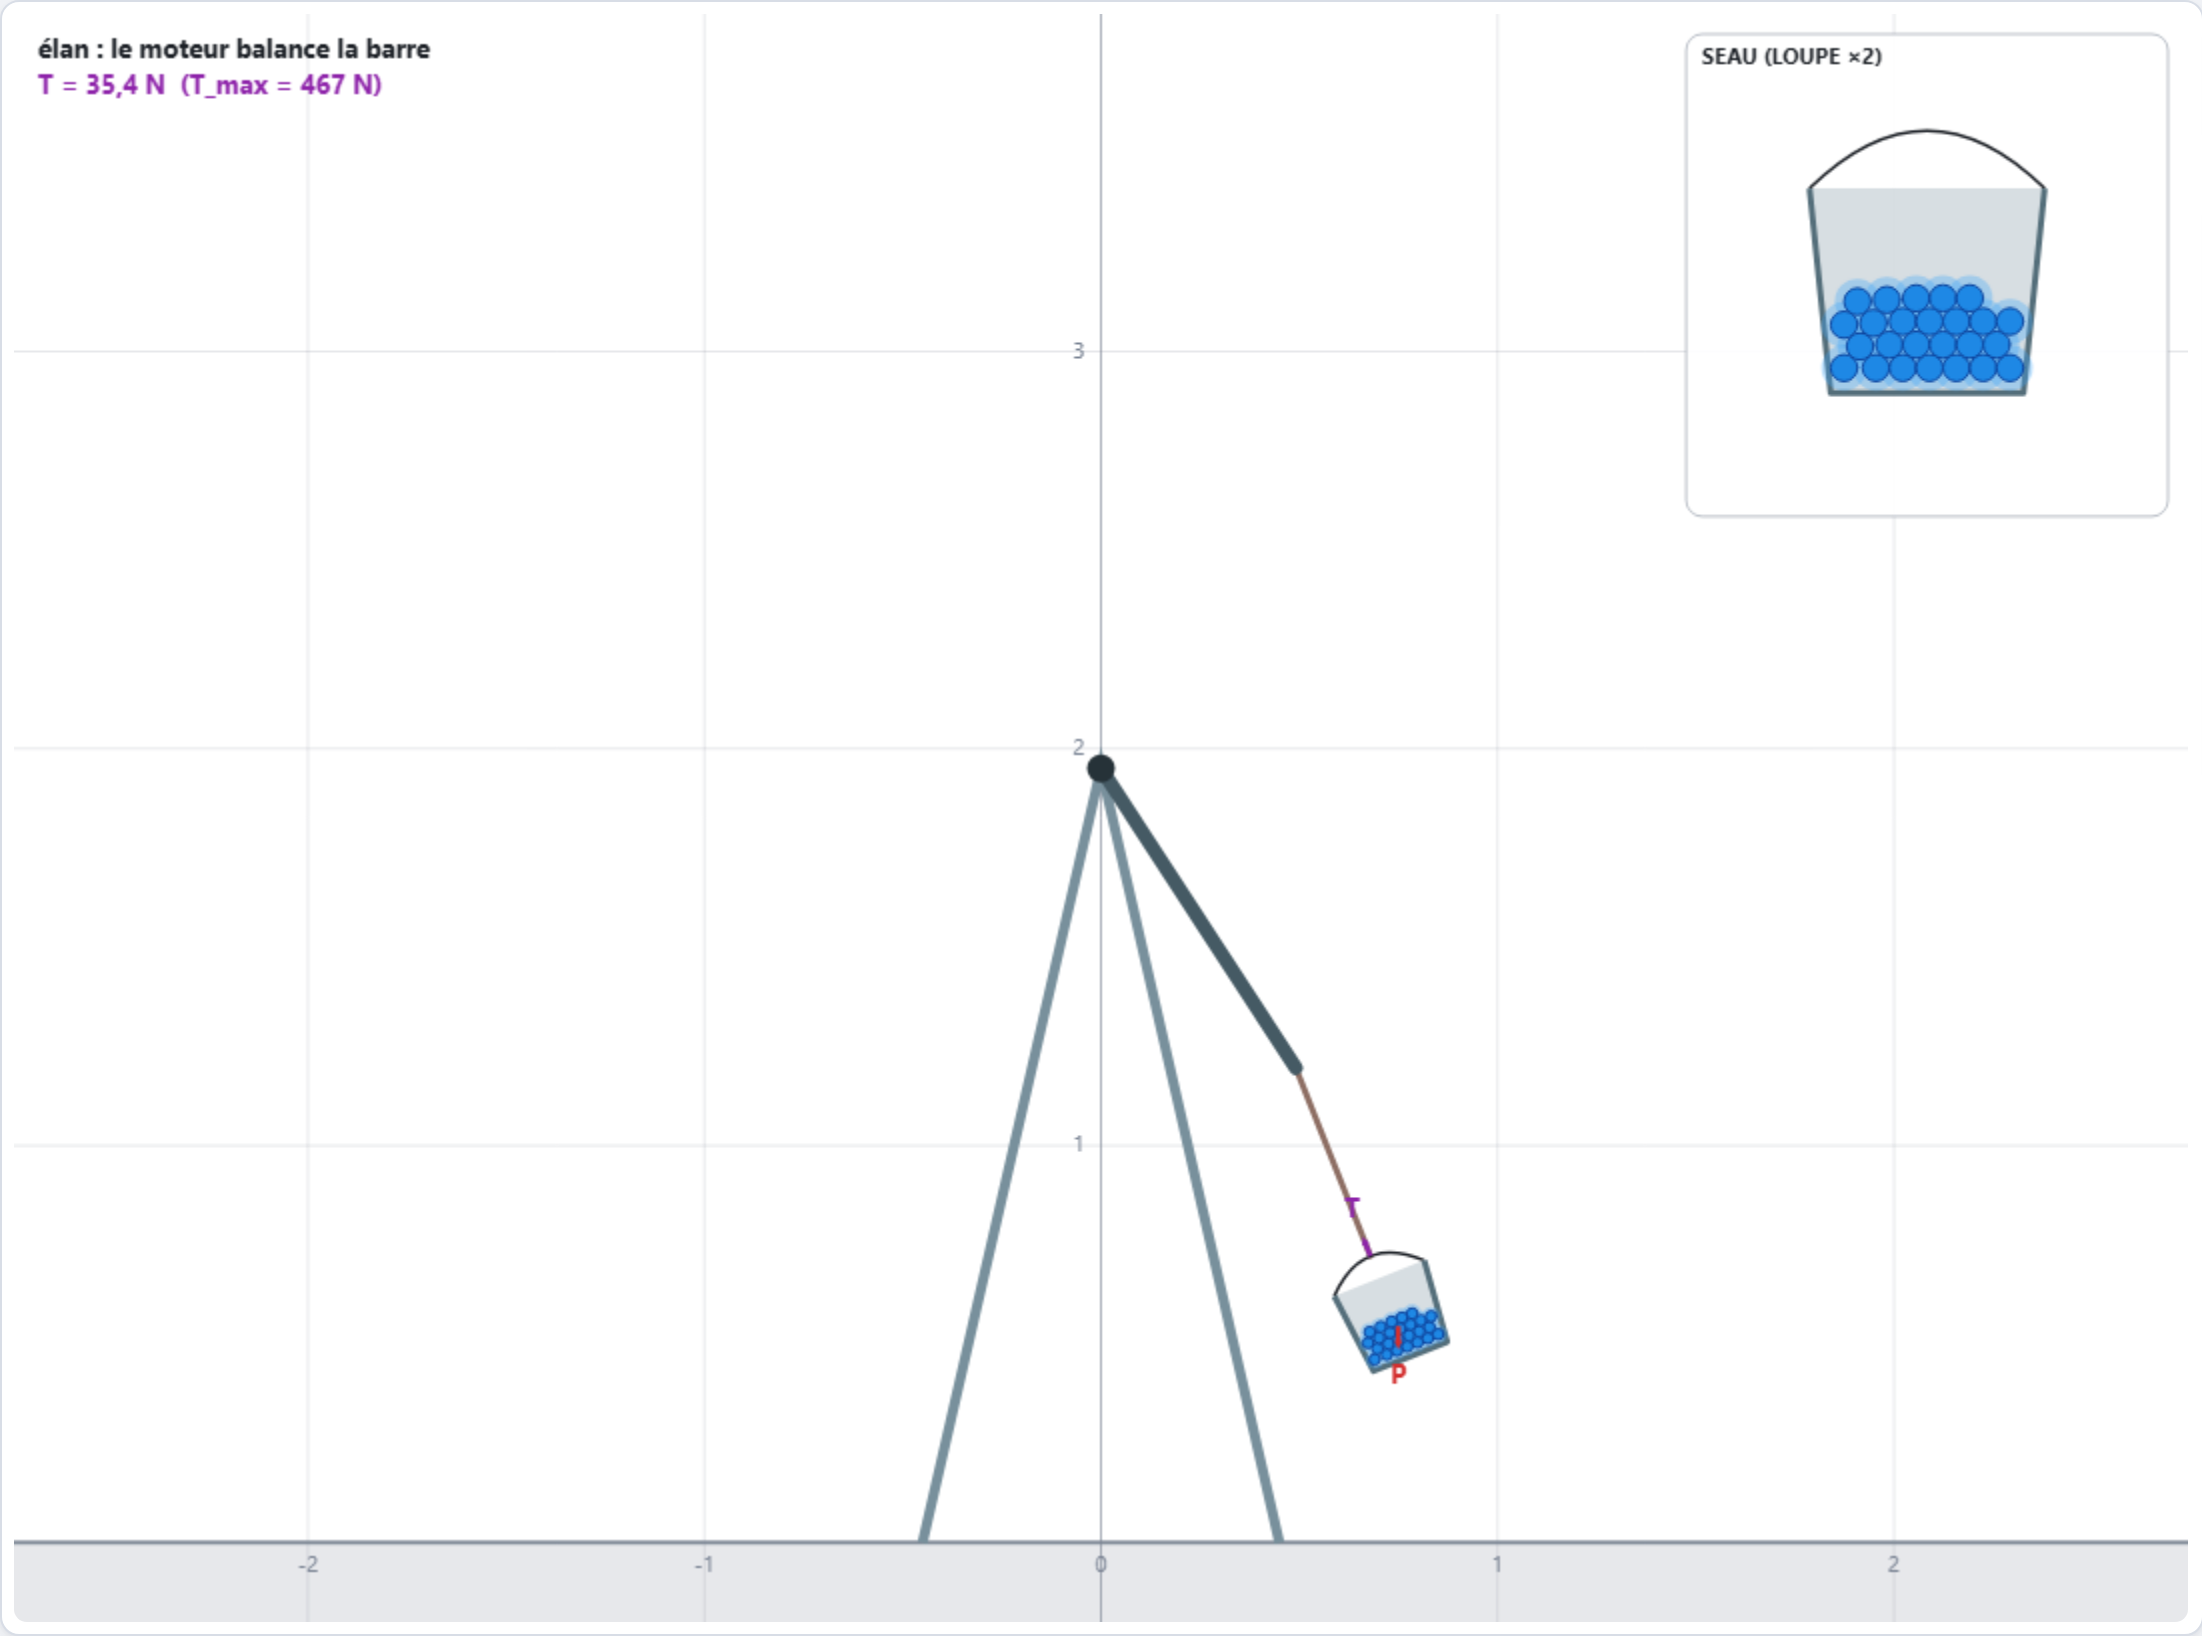
\includegraphics[width=\linewidth]{captures/jeu-elan.png}
    \caption{Élan : va-et-vient au rythme du pendule.}
  \end{subfigure}\hfill
  \begin{subfigure}[b]{0.49\linewidth}
    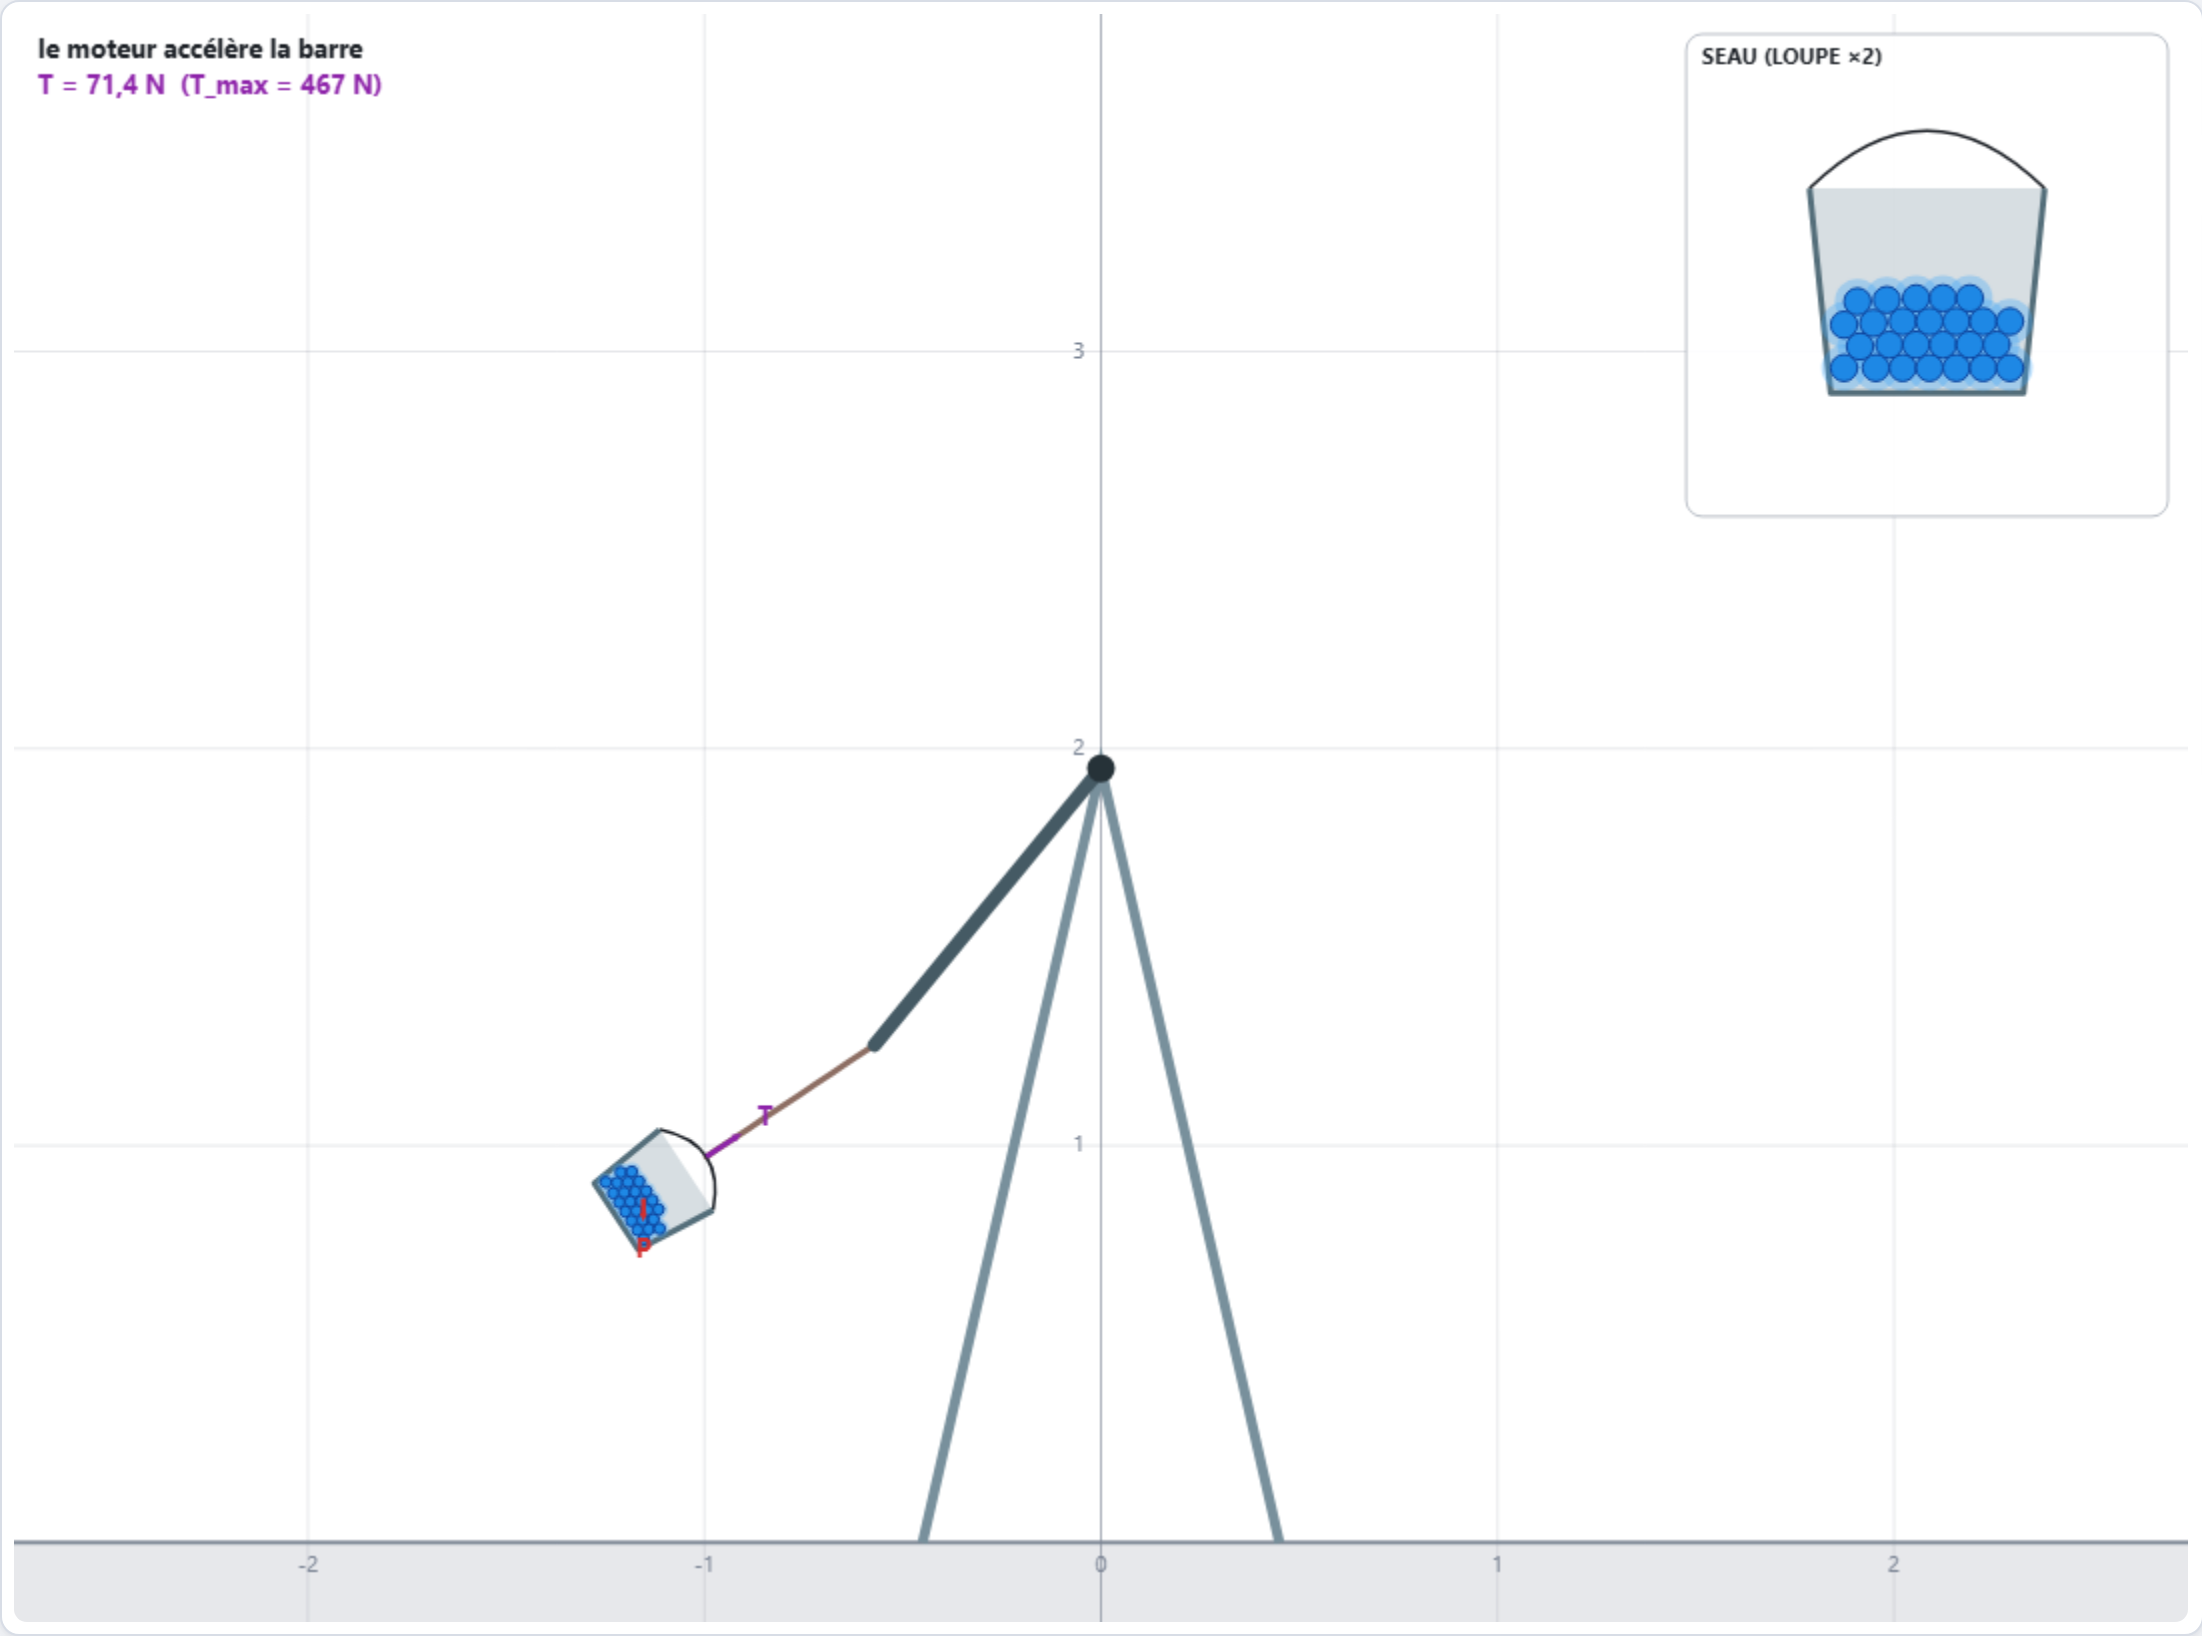
\includegraphics[width=\linewidth]{captures/jeu-lancer.png}
    \caption{Lancer : la barre devance le seau, la corde tire en biais.}
  \end{subfigure}\\[4pt]
  \begin{subfigure}[b]{0.49\linewidth}
    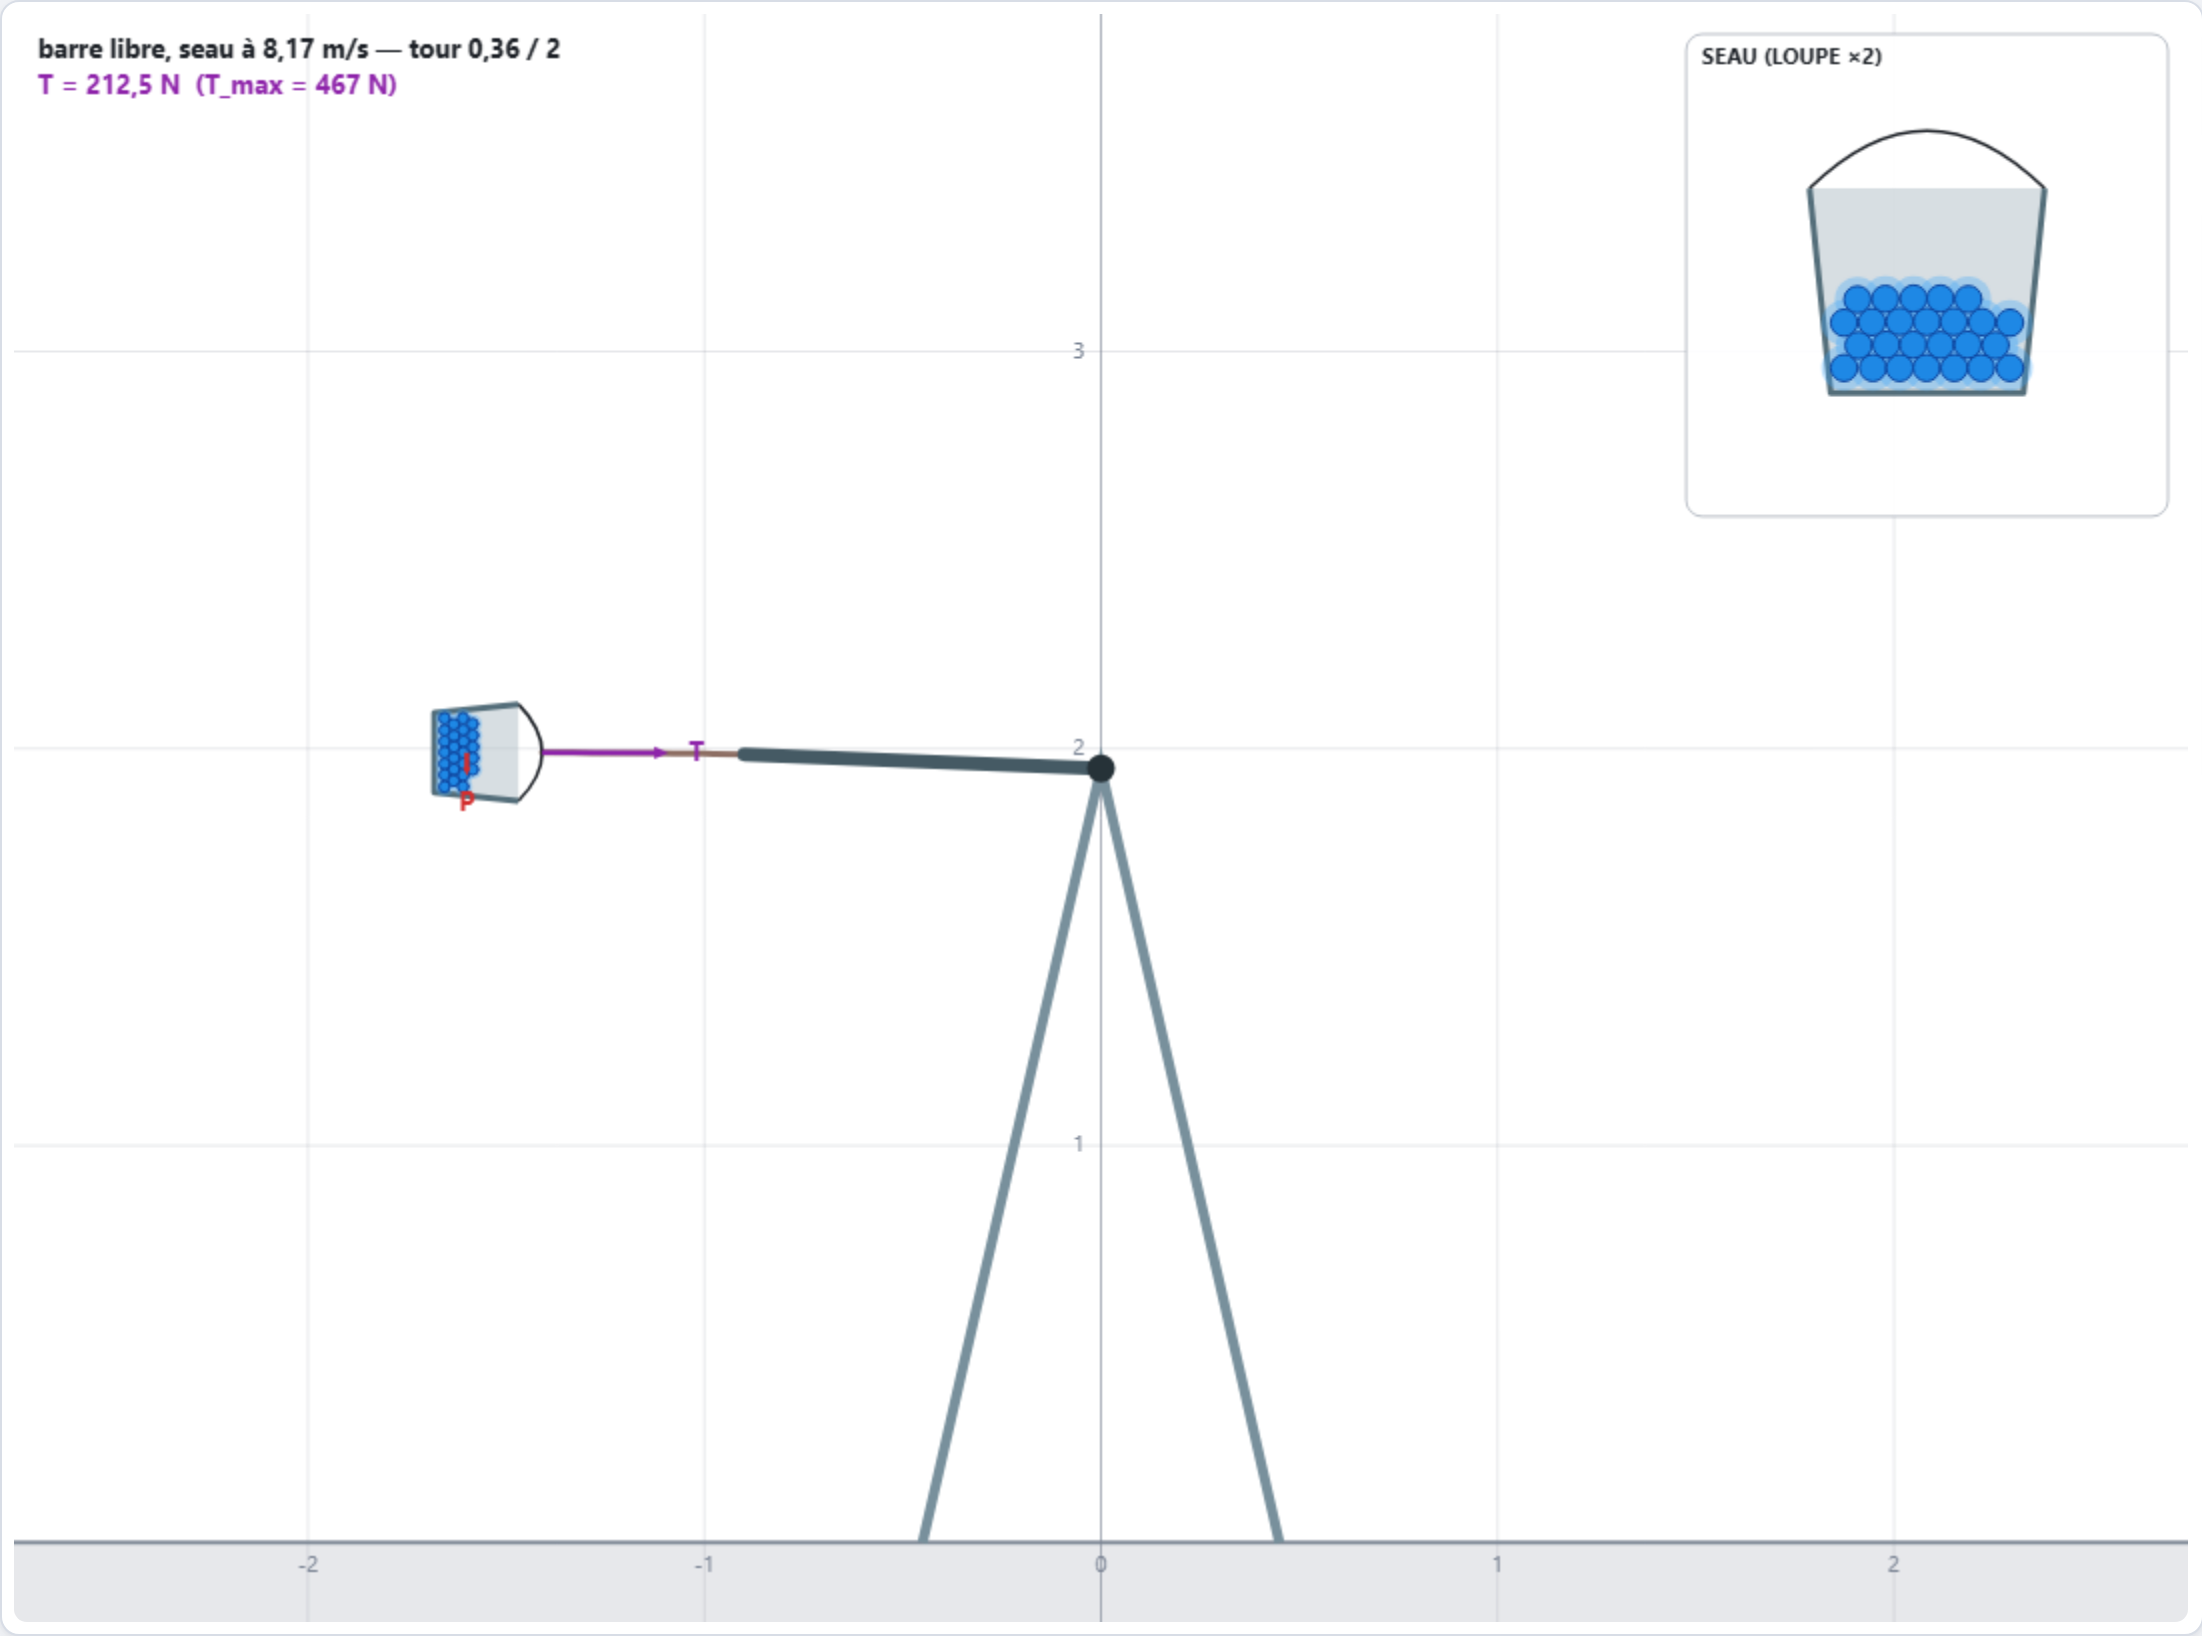
\includegraphics[width=\linewidth]{captures/jeu-tour-libre.png}
    \caption{Tour libre : chaîne alignée, eau plaquée au fond (loupe).}
  \end{subfigure}\hfill
  \begin{subfigure}[b]{0.49\linewidth}
    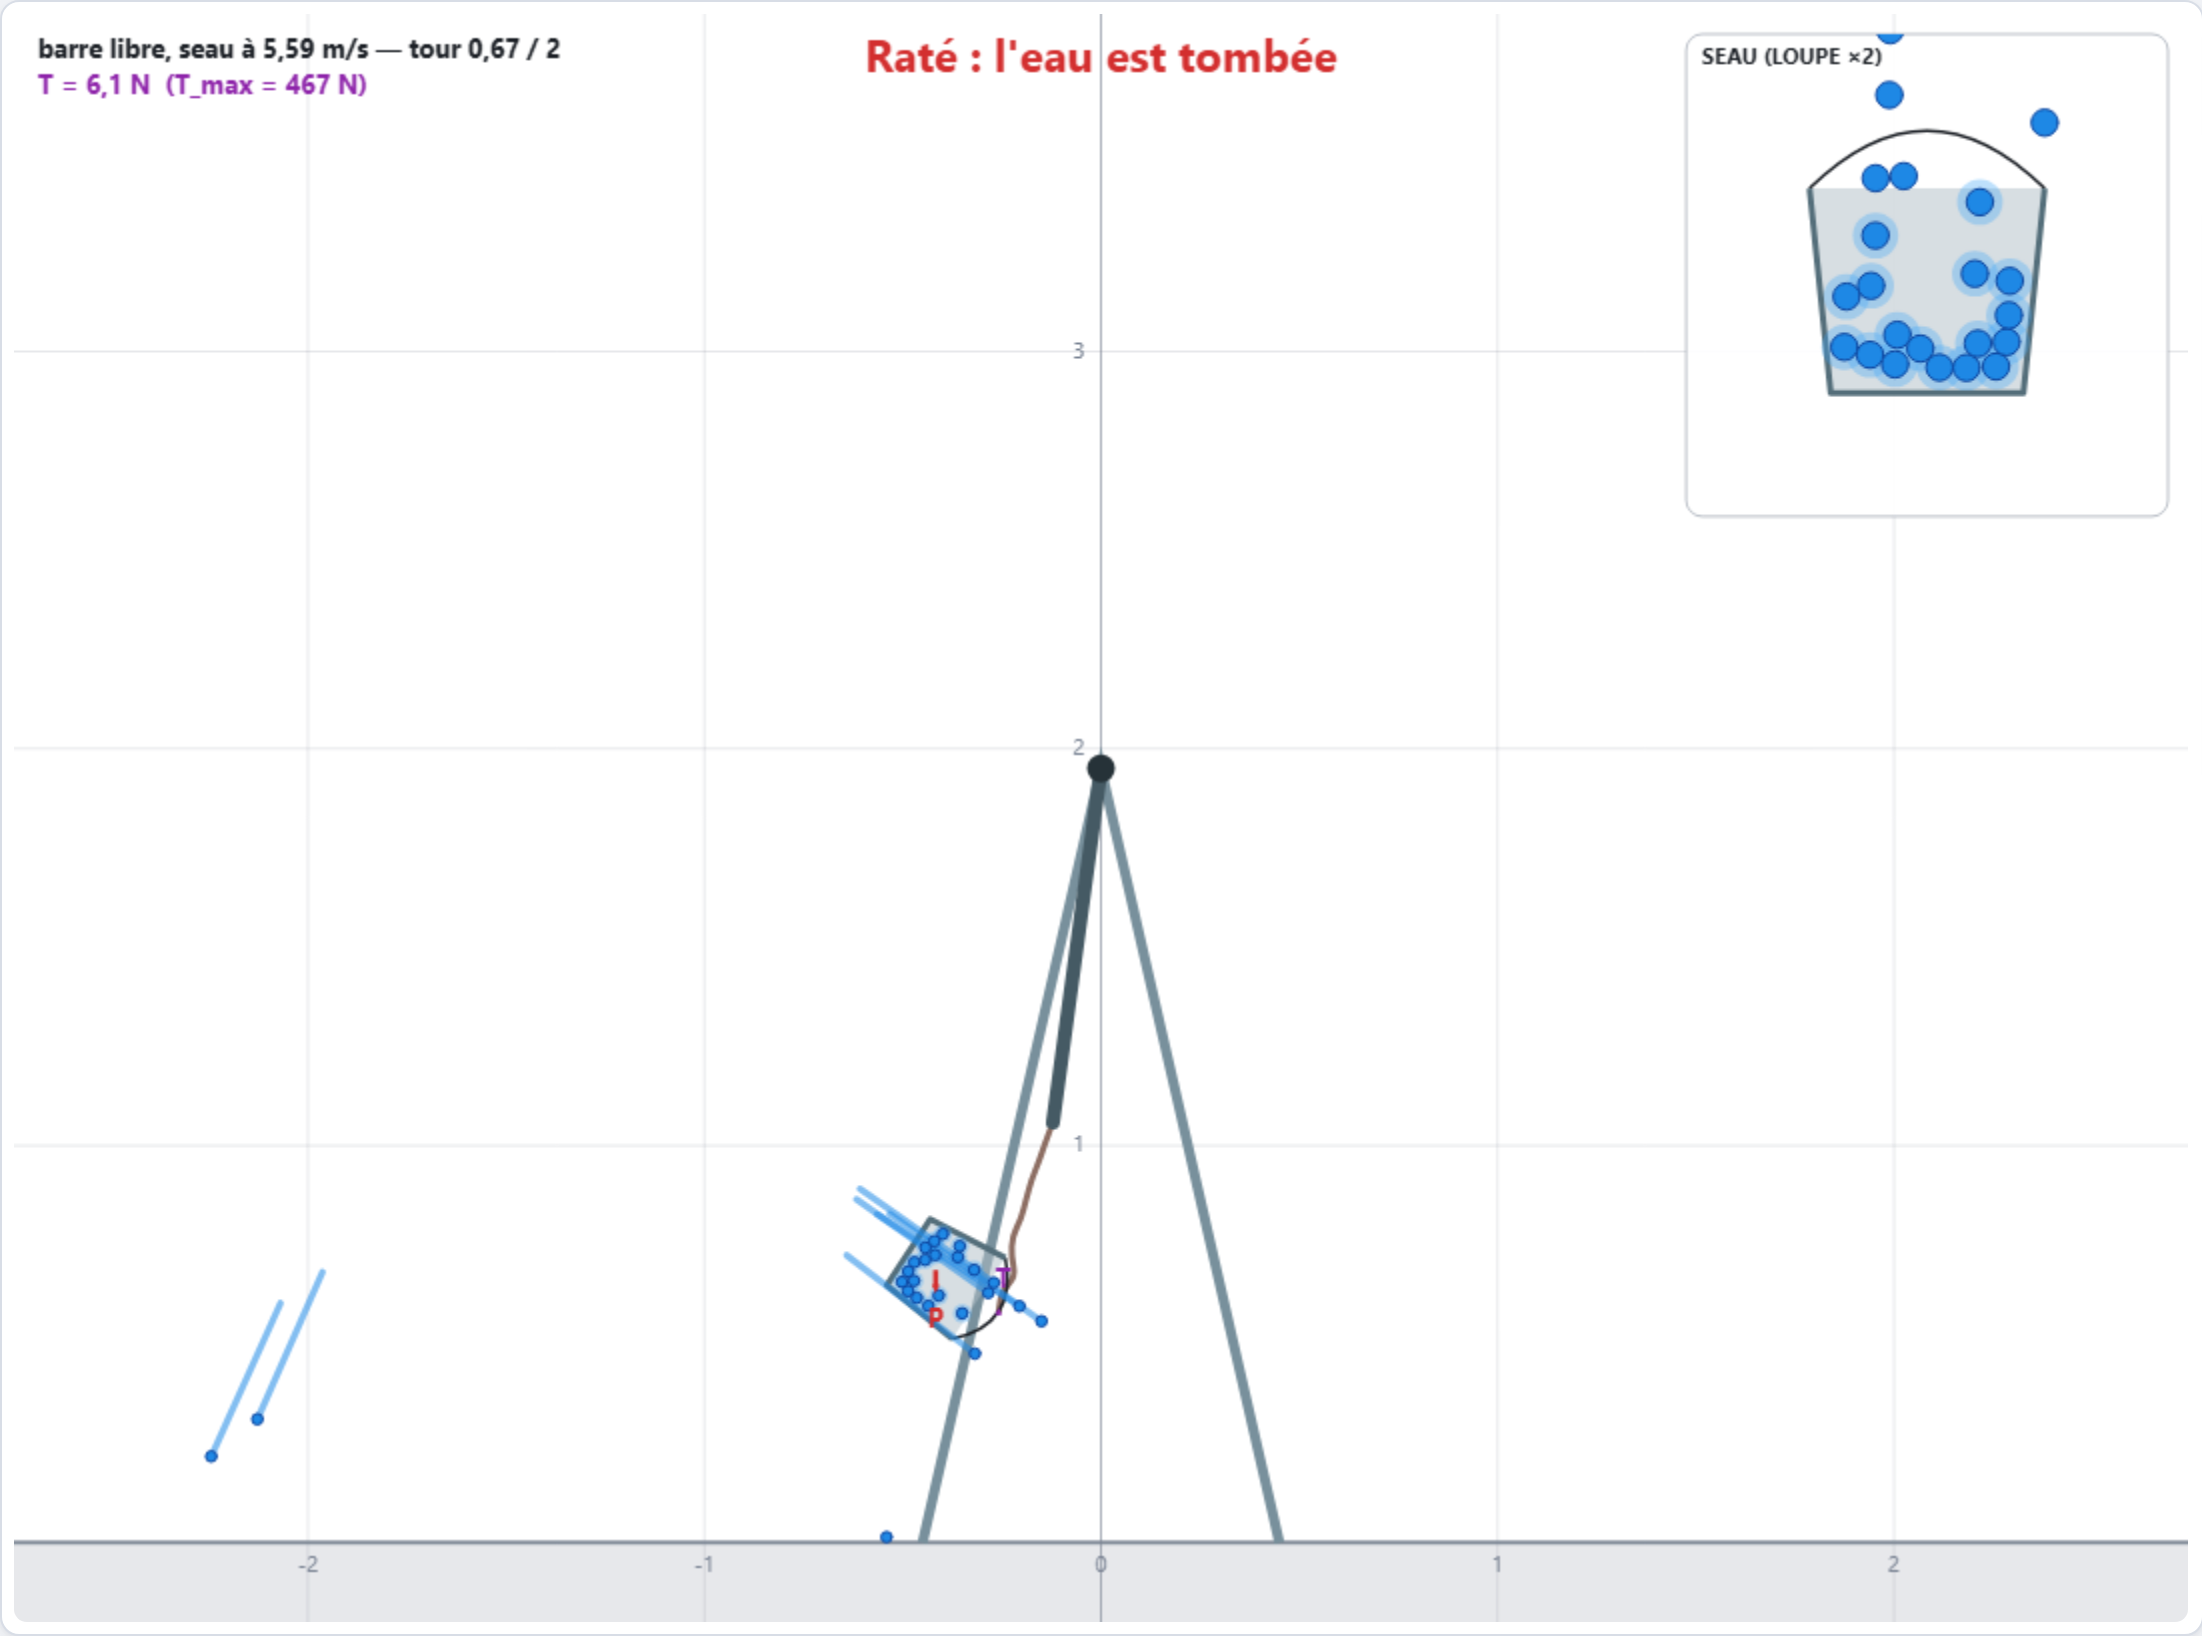
\includegraphics[width=\linewidth]{captures/jeu-rate.png}
    \caption{\(v_0 = 0{,}9 \sqrt{5 g R}\) : la corde se détend, l'eau tombe.}
  \end{subfigure}
  \caption{Captures du jeu (Terre, \(L = \SI{0,51}{m}\), \(m = \SI{4}{kg}\),
    \(T_{\max} = \SI{467}{N}\), fenêtre garantie \num{9,39} à
    \SI{11,47}{m/s}). Les vignettes (a) à (c) : \(v_0 = \SI{10,43}{m/s}\),
    réussi. En haut à droite, la loupe montre le seau dans son propre repère.}
  \label{fig-captures}
\end{figure}

\begin{figure}[!htb]
  \centering
  \begin{tikzpicture}
    \begin{axis}[width=0.78\linewidth, height=4.4cm, xlabel={\(t\) depuis le lâcher (s)}, ylabel={\(T\) (N)},
      xmin=0, grid=major, /pgf/number format/use comma, grid style={gray!20}, legend style={font=\scriptsize, at={(0.5,1.03)}, anchor=south, legend columns=2, draw=none},
      tick label style={font=\scriptsize}, label style={font=\small}]
      \addplot[tensionc, thick] table[x=t, y=simulee, col sep=comma] {figures/donnees/tension_seau.csv};
      \addplot[black, dashed] table[x=t, y=ideale, col sep=comma] {figures/donnees/tension_seau.csv};
      \legend{{simulée}, {\(m (v_0^2/R + g (3 \cos(\theta) - 2))\)}}
    \end{axis}
  \end{tikzpicture}
  \caption{Tension de la corde pendant les deux tours libres, comparée à
    l'équation~\eqref{eq-tension} (Terre, \(L = \SI{0,4}{m}\),
    \(m = \SI{2}{kg}\), \(v_0 = 1{,}15 \sqrt{5 g R} = \SI{9,83}{m/s}\)). La
    courbe idéale utilise \(v_0\) ; l'écart vient surtout de l'excès de vitesse
    au point bas et de la masse de la corde.}
  \label{fig-tension}
\end{figure}

\begin{table}[!htb]
  \centering
  \small
  \begin{tabular}{rrrrrr}
    \toprule
    \(g\) (\si{m/s^2}) & \(L\) (\si{m}) & \(m\) (\si{kg}) & \(v_0\) (\si{m/s}) & \(v_{\text{bas}}/v_0\) & \(T_{\text{pic}}/\left(m (v_0^2/R + g)\right)\) \\
    \midrule
    \num{9,81} & \num{0,2} & 5   & \num{9,55}  & \num{1,051} & \num{1,11} \\
    \num{9,81} & \num{0,4} & 2   & \num{10,26} & \num{1,057} & \num{1,15} \\
    \num{9,81} & \num{0,6} & \num{0,5} & \num{10,93} & \num{1,073} & \num{1,33} \\
    \num{3,71} & \num{0,4} & 2   & \num{6,31}  & \num{1,060} & \num{1,16} \\
    \num{1,62} & \num{0,6} & 1   & \num{4,44}  & \num{1,034} & \num{1,22} \\
    \bottomrule
  \end{tabular}
  \caption{Premier passage au point bas et pic de tension après le lâcher, pour
    \(v_0 = 1{,}2 \sqrt{5 g R}\) (vitesse estimée sur les images à
    \SI{60}{Hz}).}
  \label{tab-tours}
\end{table}

\paragraph{Limites.} Le modèle est plan, sans frottement au pivot ni résistance
de l'air. L'eau n'a pas de pression, sa viscosité est une simple traînée, et
elle ne réagit pas sur le seau ; un fluide plus réaliste (SPH ou fluides basés
sur les positions \cite{monaghan1992sph, macklin2013pbf}) n'apporterait rien à
la question posée à l'étudiant : à quelle vitesse l'eau reste-t-elle dans le
seau ? Le seau passe le point bas 3 à \SI{7}{\percent} plus vite que \(v_0\) :
le jeu est un peu plus tolérant que la formule pour la borne basse, mais plus
sévère pour la borne haute, où la tension simulée dépasse la formule. C'est
pourquoi la fenêtre garantie n'utilise que \SI{80}{\percent} de \(T_{\max}\) ;
les cinq valeurs qu'en rejoue le vérificateur réussissent toutes. Enfin,
un départ plus brutal, qui montrerait davantage la corde molle et les
éclaboussures, a été essayé : il fait tomber l'eau quel que soit \(v_0\), ce qui
rendrait les défis insolubles. Il n'a donc pas été retenu.


\FloatBarrier

\section{Conclusion}

Le jeu reproduit la condition \(v_0^2 \geq 5 g R\) du cours à 3 à
\SI{8}{\percent} près (\(k = \num{0,92}\) à \num{0,97}) avec une corde qui plie
et de l'eau en particules, sans autre action sur le seau que son poids et la
corde. Chaque défi tiré est vérifié en rejouant la simulation, et les écarts
restants (vitesse au point bas, masse de la corde, taille du seau) sont
expliqués et couverts par les marges de la fenêtre garantie.


\printbibliography[title={Bibliographie}]

\end{document}
